% fig_oc_tripping_curves.tex
% TR-40: Standard inverse time-current curves for Group 1 and Group 2
%
% IEC Standard Inverse: t = TMS * 0.14 / (M^0.02 - 1)  where M = I/Ip
%
% Group 1: Ip=1.50, TMS=0.10  → curves for grid-connected
% Group 2: Ip=0.30, TMS=0.20  → curves for islanded
%
% X-axis: I [pu]  (log scale 0.1 to 30)
% Y-axis: t [s]   (log scale 0.1 to 10)
%
% Key operating points:
%   GC mid-line fault at 22.2 pu → Group 1: ~0.23 s
%   IS mid-line fault at  8.0 pu → Group 2: ~0.41 s
%   IS far-end fault at   4.0 pu → Group 2: ~0.53 s

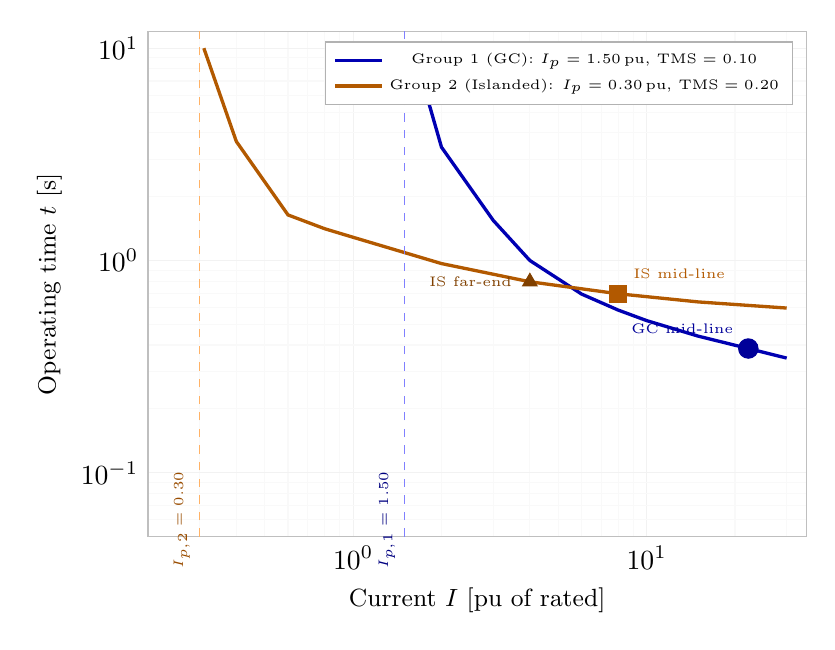
\begin{tikzpicture}
\begin{loglogaxis}[
  name         = tcax,
  width        = 0.82\textwidth,
  height       = 8.0cm,
  xlabel       = {Current $I$ [pu of rated]},
  ylabel       = {Operating time $t$ [s]},
  xlabel style = {font=\small},
  ylabel style = {font=\small},
  xmin=0.2, xmax=35,
  ymin=0.05, ymax=12,
  tick style   = {draw=none},
  axis line style={gray!50},
  grid         = both,
  grid style   = {gray!10},
  minor grid style={gray!5},
  legend style = {at={(0.98,0.98)}, anchor=north east, font=\tiny,
                  draw=gray!60, fill=white},
  clip=false,
]

%% Group 1: Ip=1.50, TMS=0.10, SI curve
%% t = 0.10 * 0.14 / (M^0.02 - 1)  with M = I/1.5
\addplot[blue!70!black, very thick]
  coordinates {
    (1.60, 10.000)
    (2.00,  3.418)
    (3.00,  1.546)
    (4.00,  1.000)
    (6.00,  0.695)
    (8.00,  0.584)
    (10.0,  0.521)
    (15.0,  0.440)
    (22.2,  0.385)
    (30.0,  0.347)
  };
\addlegendentry{Group 1 (GC): $I_p=1.50$\,pu, $\mathrm{TMS}=0.10$}

%% Group 2: Ip=0.30, TMS=0.20, SI curve
%% t = 0.20 * 0.14 / (M^0.02 - 1)  with M = I/0.3
\addplot[orange!70!black, very thick]
  coordinates {
    (0.31, 10.000)
    (0.40,  3.636)
    (0.60,  1.639)
    (0.80,  1.411)
    (1.00,  1.286)
    (2.00,  0.967)
    (4.00,  0.794)
    (8.00,  0.697)
    (15.0,  0.638)
    (30.0,  0.597)
  };
\addlegendentry{Group 2 (Islanded): $I_p=0.30$\,pu, $\mathrm{TMS}=0.20$}

%% Operating points
% GC mid-line fault: I=22.2, t=0.385 (Group 1)
\addplot[blue!60!black, only marks, mark=*, mark size=3.5pt]
  coordinates {(22.2, 0.385)};
\node[blue!60!black, font=\tiny, above left=2pt] at (axis cs:22.2, 0.385)
  {GC mid-line};

% IS mid-line fault: I=8.0, t=0.697 (Group 2)
\addplot[orange!70!black, only marks, mark=square*, mark size=3pt]
  coordinates {(8.0, 0.697)};
\node[orange!70!black, font=\tiny, above right=2pt] at (axis cs:8.0, 0.697)
  {IS mid-line};

% IS far-end fault: I=4.0, t=0.794 (Group 2)
\addplot[orange!50!black, only marks, mark=triangle*, mark size=3pt]
  coordinates {(4.0, 0.794)};
\node[orange!50!black, font=\tiny, left=3pt] at (axis cs:4.0, 0.794)
  {IS far-end};

%% Pickup markers
\draw[blue!50, thin, dashed]
  (axis cs:1.50, 0.05) -- (axis cs:1.50, 12);
\node[blue!50!black, font=\tiny, rotate=90, anchor=south] at (axis cs:1.50, 0.06)
  {$I_{p,1}=1.50$};

\draw[orange!60, thin, dashed]
  (axis cs:0.30, 0.05) -- (axis cs:0.30, 12);
\node[orange!60!black, font=\tiny, rotate=90, anchor=south] at (axis cs:0.30, 0.06)
  {$I_{p,2}=0.30$};

\end{loglogaxis}
\end{tikzpicture}
